\section{Experiments and results}\label{experiments}

\subsection{New models and embeddings}
 In this project, several embedding models were tested, but it was soon rather clear that the best results will be obtained by the most complex embedding models. Additionally, we wanted to decrease the input size of classifiers to reduce the training time and complexity of several models. Described goals were achieved by introducing new embedding models with aggregated word embeddings. Said models are \texttt{DistilBERT} and \texttt{SentenceTransformerMPNET} with word embeddings transformed to singular sentence embedding, by aggregating them. This seemingly minor change greatly increased accuracy scores across all classifiers and set a new standard for future experiments.

 We also used two new classifiers: DenseNet which consists of a few fully connected dense layers, and the 2-step CNN closer described before. 
 
 Results of our experiments on a balanced dataset are visible in \ref{tab:distilbert_results} and \ref{tab:mpnet_results} tables. $\Delta$ Acc. signify the difference between results acquired in this project for this dataset with the new embedding and the best results obtained in the previous project.

\begin{table}[!h]
\centering
\begin{tabular}{l|l|l|l}
\textbf{Classifier} & \textbf{Accuracy} & \textbf{F1-score} & \textbf{ $\Delta$ Acc.}  \\ \hline
NB         & 54.40\%           & 53.16\%           & + 11.16               \\
SVM          & 62.06\%           & 61.07\%           & + 11.45               \\
XGBoost             & 63.93\%           & 63.78\%           & \textbf{+ 18.46}      \\
\textbf{CNN}        & \textbf{65.47\%}  & \textbf{65.53\%}  & + 8.99                \\
DenseNet            & 64.96\%           & 64.99\%           & \multicolumn{1}{c}{-} \\
2StepCNN            & 62.21\%           & 57.97\%           & \multicolumn{1}{c}{-}
\end{tabular}
\caption{Results for the DistilBERT  on balanced dataset}
\label{tab:distilbert_results}
\end{table}

\begin{table}[!h]
\centering
\begin{tabular}{l|l|l|l}
\textbf{Classifier} & \textbf{Accuracy} & \textbf{F1-score} & \textbf{$\Delta$ Acc.}  \\ \hline
NB         & 56.23\%           & 55.97\%           & + 12.99               \\
SVM          & 62.83\%           & 61.66\%           & + 12.22               \\
XGBoost             & 62.45\%           & 62.31\%           & \textbf{+ 16.98}      \\
CNN                 & 65.06\%           & 64.30\%           & + 8.58                \\
\textbf{DenseNet}   & \textbf{66.42\%}  & \textbf{66.08\%}  & \multicolumn{1}{c}{-} \\
2StepCNN            & 63.34\%           & 60.44\%           & \multicolumn{1}{c}{-}
\end{tabular}
\caption{Results for the SentenceTransformerMPNET on balanced dataset}
\label{tab:mpnet_results}
\end{table}

As we can see, all results are significantly better than in the previous project which shows how important embedding is in text classification. Also, the new classifier DenseNet gives very good results, even given its quite simple structure. The comparison of the results is shown in Figure \ref{fig:embed_comparison}.

\subsection{Fine-tunning embedding models}
The natural next step was to improve the information contained in the embedding model by combining it with the classification layer and fine-tuning the combined architecture. Since a DistilBERT was pre-trained on a broad corpus and a wide range of texts, we hoped that by partially training it on lyrics it will be able to improve the quality of the created embeddings.  This task was realized on \texttt{small\_balanced} version of the available dataset. Unfortunately, repeated experiments did not bring the expected results and the model performance was not significantly improved. A comparison of both fine-tuned  and pre-trained models is presented in Table \ref{tab:tuning_results}. Lack of improvement may indicate problems in the training process but repeated experiments and tests on different models indicate that this was not the case. 


\begin{table}[h]
\centering
\begin{tabular}{l|r|r|r}
 \textbf{Embedding} & \textbf{Classifier} & \textbf{Accuracy} & \textbf{F1 score} \\\hline
pretrained & Dense & 0.6455 & 0.6431 \\
fine-tuned & Dense & \textbf{0.65} & \textbf{0.6682} \\
\end{tabular}
\caption{Results after fine-tuning}
\label{tab:tuning_results}
\end{table}

\subsection{Addition of sentiment analysis}
One of the main things that we wanted to test, was the impact of additional information added to the embeddings. At the same time since one of the assumptions of the project was working with only the lyrics, features that we could add to the embedding of the lyrics are all lyrics based. Our idea was to incorporate sentiment obtained by a separate model. Unfortunately, since we focused on using as hardware demanding embedding model there were little to no resources left for this sentiment model. After minor research we settled for \href{https://huggingface.co/gokuls/BERT-tiny-emotion-intent}{\texttt{BERT-tiny-emotion-intent}} model. It offers sentiment prediction in form of a six-dimensional vector measuring the sentiment as happy, sad, neutral, angry, excited, or frustrated. This is to some extent a redundancy since we expect the sentiment to be present in embeddings, at least to some degree, but this information may not be easy for the model to extract especially since our classification models are relatively simple.

We tested the influence of sentiment in two experiments. The first one was oriented on the changes in the performance of classifiers. As it can be seen in \ref{tab:sentiment_results} results for feature vector enriched with embeddings did not really change, when compared to \ref{tab:distilbert_results}. The only exception here is the XGBoost model which improved significantly, but this may be partially explained by the instability of the XGBoost which was observed. 

\begin{table}[h]
\centering
\begin{tabular}{l|r|r|r}
 \textbf{Classifier} & \textbf{Accuracy} & \textbf{Bal. Acc.} & \textbf{F1 score} \\\hline
Naive Bayes & 0.5272 & 0.5272 & 0.5095 \\
Linear SVM & 0.6054 & 0.6054 & 0.5998 \\
XGBoost & 0.6300 & 0.6300 & 0.6279 \\
CNN & 0.6433 & 0.6433 & \textbf{0.6433} \\
Dense & \textbf{0.6449} & \textbf{0.6449} & 0.6341 \\
\end{tabular}
\caption{Classification results for better embeddings }
\label{tab:sentiment_results}
\end{table}

The second experiment concerning sentiment included fine-tuning the combination of the embedding model, sentiment model and dense classifier. Same as with the previous first fine-tuning the results did not really change \ref{tab:sentiment_tuning_results}, and actually the model without sentiment achieves the best score, but only by a small margin of less than 1\%. 

\begin{table}[h]
\centering
\begin{tabular}{l|r|r}
 \textbf{sentiment}& \textbf{Accuracy} & \textbf{F1 score} \\\hline
yes &  0.6412 & 0.6638 \\
no &  \textbf{0.65} & \textbf{0.6682} \\
\end{tabular}
\caption{Results after fine-tuning with or without sentiment}
\label{tab:sentiment_tuning_results}
\end{table}

\subsection{Division into two models}

There were already shown some results for the 2-step CNN classifier on the balanced dataset in the previous section in tables \ref{tab:distilbert_results} and \ref{tab:mpnet_results}. In general, achieved by 2-step CNN accuracies were slightly worse than those of normal CNN and DenseNet.

But this classifier was created with the thought of an unbalanced dataset and therefore results on this dataset are the most important to us.  Therefore, we tested 2-step CNN and two other classifiers which gave the best results in previous tests on the unbalanced dataset (which is also much bigger than balanced) to see if separate recognition of the biggest class gives better results. Results are in Table \ref{tab:unbalanced_results_2_step} and the comparison is shown in Figure \ref{fig:metric_comparison}.

\begin{table}[!h]
\centering
\begin{tabular}{l|l|l|l}
\textbf{CLassifier} & \textbf{Accuracy} & \textbf{Bal. acc.} & \textbf{F1 score} \\ \hline
CNN                 & 64.74\%           & 50.71\%                & 60.88\%           \\
\textbf{NN}         & \textbf{65.23\%}  & 53.08\%                & \textbf{62.14\%}  \\
\textbf{2-step CNN} & 52.94\%           & \textbf{59.88\%}       & \textbf{54.11\%} 
\end{tabular}
\caption{Results for 2-step CNN, DenseNet, and CNN for DistilBERT on unbalanced dataset}
\label{tab:unbalanced_results_2_step}
\end{table}

Even though neither accuracy nor F1-score was better for 2-Step CNN, it proved to give higher balanced accuracy results. Therefore it may be better than other classifiers depending on the task at hand.

\subsection{Creation of the dataset}
We conducted multiple tests for our dataset as it was a lot smaller than the other ones. The results are presented in Tables \ref{tab:dataset_res}, \ref{tab:dataset_res_norm} and Figures \ref{fig:acc_dataset}, \ref{fig:f1_dataset}, \ref{fig:acc_dataset_norm}, \ref{fig:f1_dataset_norm}. The best embedding turned out to be DistilBERT. But when it comes to classifiers the results were quite similar so it makes more sense to use the most basic classifier to limit the computations.

\onecolumn



\begin{figure}
\centering
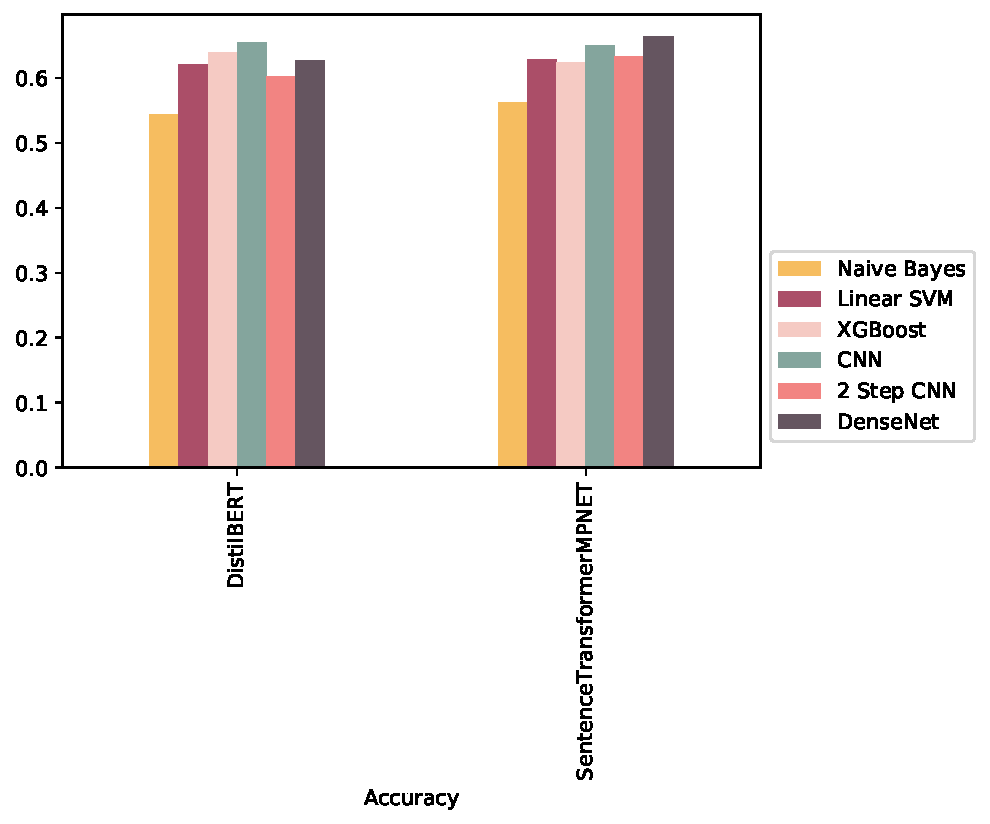
\includegraphics[width=0.8\linewidth]{plots/accuracy_small_balanced.pdf}
\caption{Comparison of DistilBERT and SentenceTransformerMPNET on balanced dataset}
\label{fig:embed_comparison}
\end{figure}


\begin{figure}
\centering
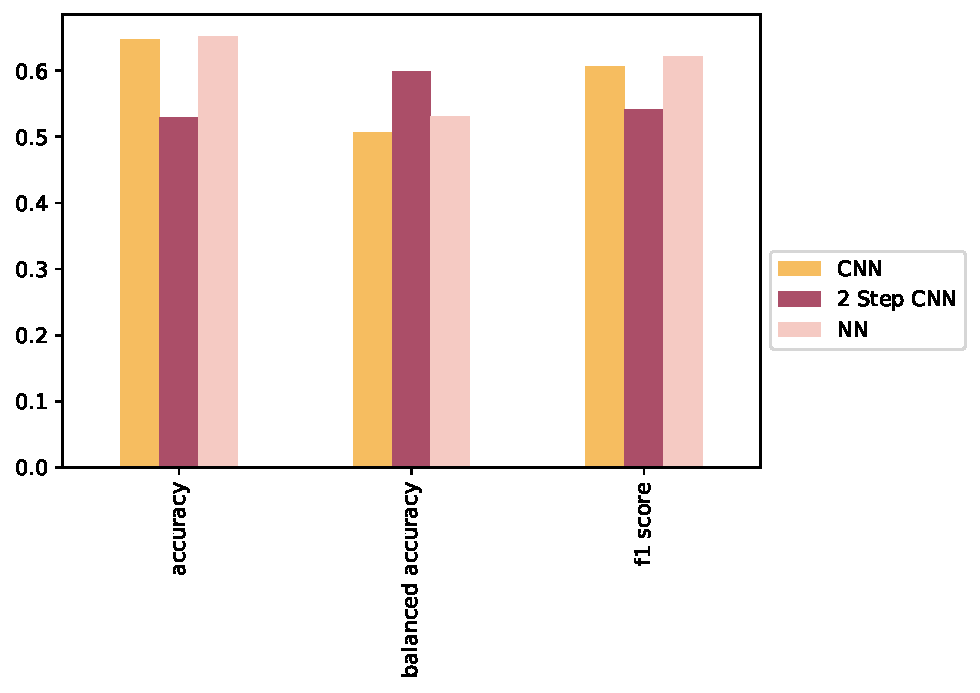
\includegraphics[width=0.8\linewidth]{plots/metrics_comparison_small.pdf}
\caption{Comparison of different metrics for different classifiers on unbalanced dataset}
\label{fig:metric_comparison}
\end{figure}

\begin{table}[h]
\centering
\begin{tabular}{l|l|r|r}
\textbf{Embedding} & \textbf{Classifier} & \textbf{Accuracy} & \textbf{F1 score} \\\hline
Smaller BERT & Naive Bayes & 0.379479 & 0.328668 \\
Smaller BERT & Linear SVM & 0.399837 & 0.353035 \\
Smaller BERT & XGBoost & 0.375407 & 0.374183 \\
Smaller BERT & CNN & 0.415309 & 0.401595 \\
Glove & Naive Bayes & 0.333876 & 0.259667 \\
Glove & Linear SVM & 0.320033 & 0.295821 \\
Glove & XGBoost & 0.343648 & 0.336383 \\
Glove & CNN & 0.374593 & 0.382742 \\
\textbf{DistilBERT} & \textbf{Naive Bayes} & \textbf{0.547231} & \textbf{0.550679} \\
DistilBERT & Linear SVM & 0.477199 & 0.373867 \\
DistilBERT & XGBoost & 0.518730 & 0.519839 \\
DistilBERT & CNN & 0.535016 & 0.530048 \\
DistilBERT & DenseNet & 0.516287 & 0.516995 \\
SentenceTransformerMPNET & CNN & 0.495928 & 0.499407 \\
SentenceTransformerMPNET & DenseNet & 0.517915 & 0.517484 \\
\end{tabular}
\caption{Results for the created dataset and unnormalized lyrics}
\label{tab:dataset_res}
\end{table}

\begin{figure}
\centering
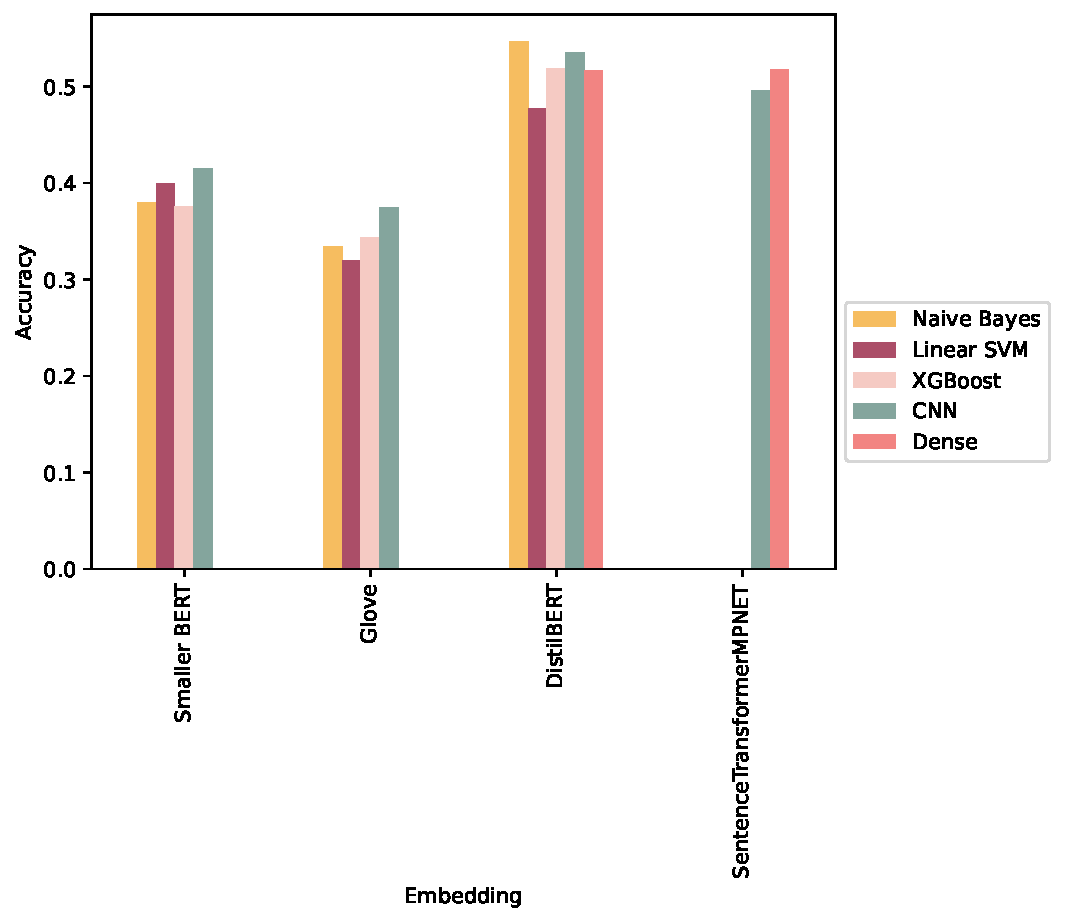
\includegraphics[width=0.8\linewidth]{plots/accuracy_dataset.pdf}
\caption{Accuracy for the created dataset and unnormalized lyrics}
\label{fig:acc_dataset}
\end{figure}

\begin{figure}
\centering
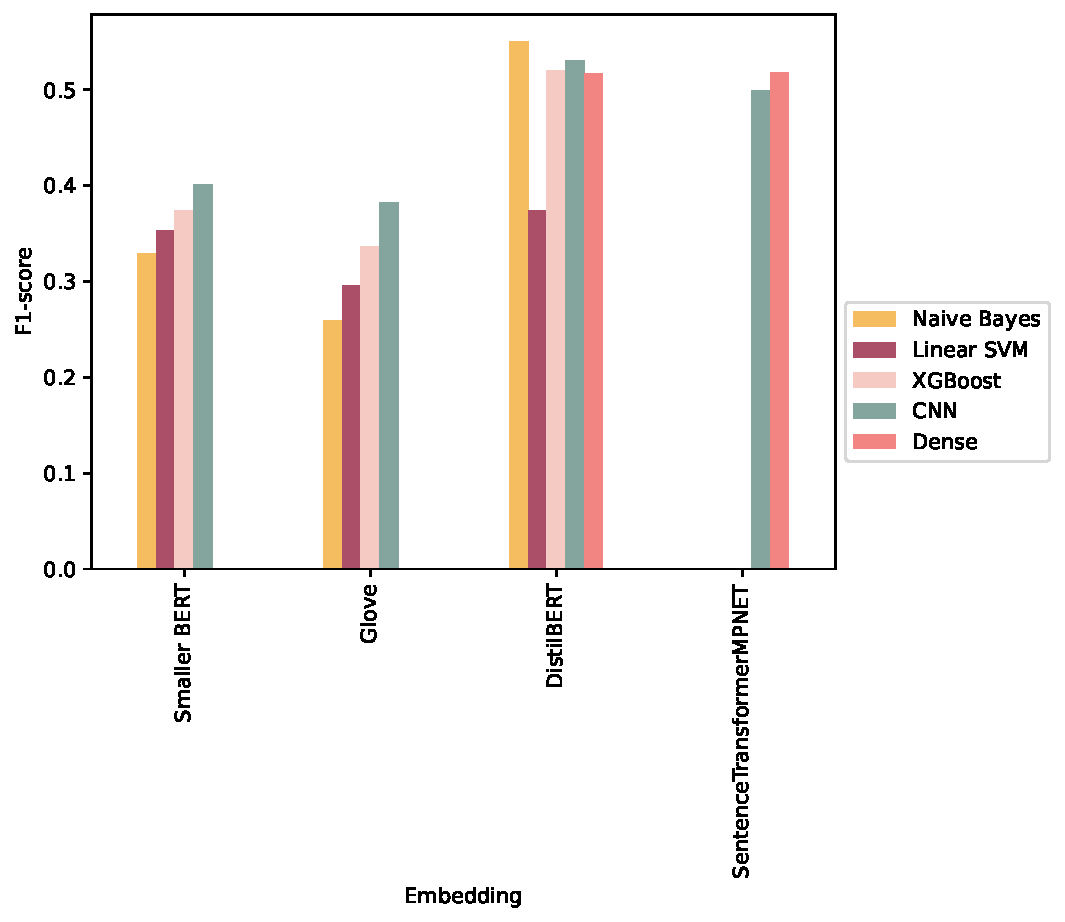
\includegraphics[width=0.8\linewidth]{plots/f1_dataset.pdf}
\caption{F1-score for the created dataset and unnormalized lyrics}
\label{fig:f1_dataset}
\end{figure}

\begin{table}[h]
\centering
\begin{tabular}{l|l|r|r}
\textbf{Embedding} & \textbf{Classifier} & \textbf{Accuracy} & \textbf{F1 score} \\\hline
Smaller BERT & Naive Bayes & 0.310261 & 0.247440 \\
Smaller BERT & Linear SVM & 0.368078 & 0.352763 \\
Smaller BERT & XGBoost & 0.400651 & 0.395027 \\
Smaller BERT & CNN & 0.439739 & 0.439537 \\
Glove & Naive Bayes & 0.328176 & 0.236727 \\
Glove & Linear SVM & 0.383550 & 0.376734 \\
Glove & XGBoost & 0.372964 & 0.369424 \\
Glove & CNN & 0.389251 & 0.395433 \\
DistilBERT & Naive Bayes & 0.515472 & 0.495294 \\
DistilBERT & Linear SVM & \textbf{0.541531} & 0.492267 \\
DistilBERT & XGBoost & 0.503257 & 0.500318 \\
DistilBERT & CNN & 0.494300 & 0.494112 \\
DistilBERT & DenseNet & 0.518730 & \textbf{0.517378} \\
SentenceTransformerMPNET & CNN & 0.514658 & 0.509839 \\
SentenceTransformerMPNET & DenseNet & 0.500000 & 0.501151 \\
\end{tabular}
\caption{Results for the created dataset and normalized lyrics}
\label{tab:dataset_res_norm}
\end{table}

\begin{figure}
\centering
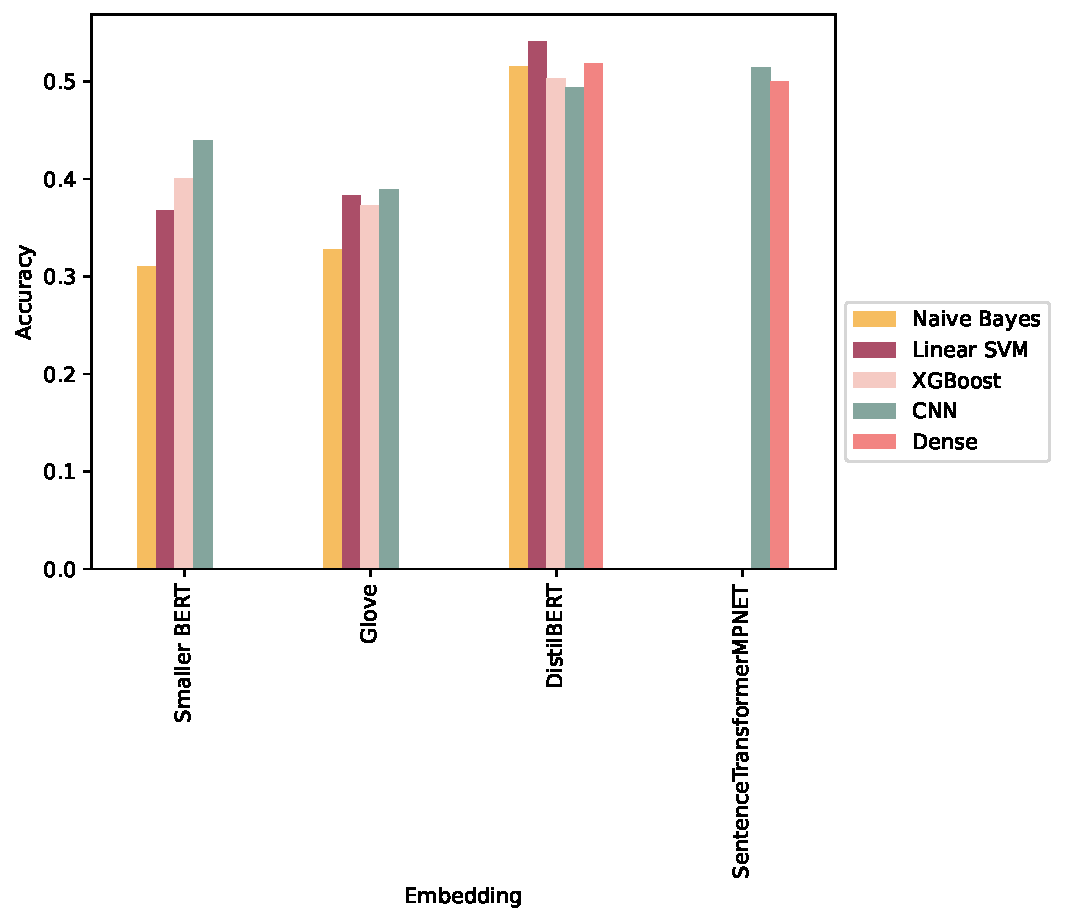
\includegraphics[width=0.8\linewidth]{plots/accuracy_dataset_norm.pdf}
\caption{Accuracy for the created dataset and normalized lyrics}
\label{fig:acc_dataset_norm}
\end{figure}

\begin{figure}
\centering
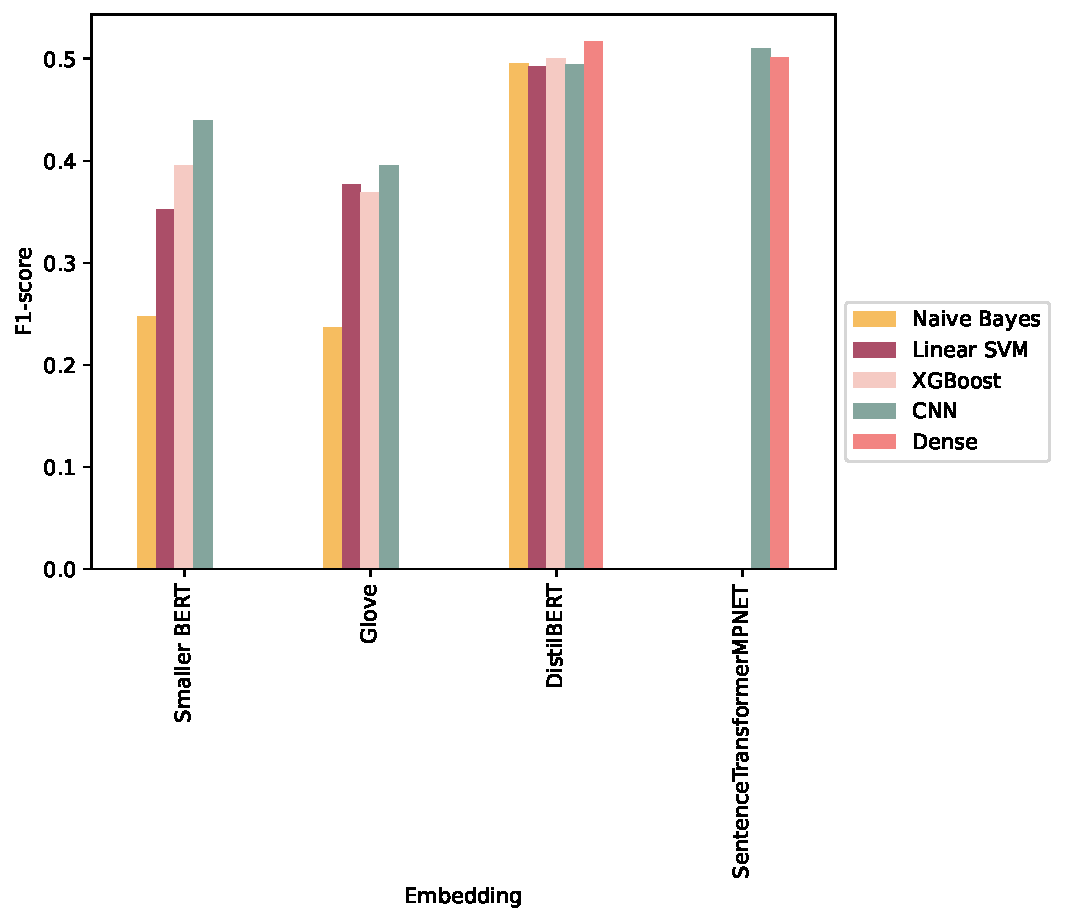
\includegraphics[width=0.8\linewidth]{plots/f1_dataset_norm.pdf}
\caption{F1-score for the created dataset and normalized lyrics}
\label{fig:f1_dataset_norm}
\end{figure}
\twocolumn